% Généré par build_draft.py. Maquette de travail, non destinée à l'impression finale.
\documentclass[final]{beamer}
\usepackage[orientation=portrait,size=a0,scale=1.0]{beamerposter}
\usepackage{graphicx,booktabs,tikz,pgfplots,anyfontsize}
\usepackage{qrcode}
\pgfplotsset{compat=1.14}
% Thème du template fourni, intégré pour conserver un document autonome.
\makeatletter

% ====================
% Dependencies
% ====================

\RequirePackage{exscale}
\RequirePackage{ragged2e}
\RequirePackage{changepage}
\RequirePackage{fontspec}
\RequirePackage{calc}

% ====================
% Fonts
% ====================

% Même familles et graisses que le template ; noms de fichiers TeX portables.
\newfontfamily\Raleway[Ligatures=TeX,Extension=.otf,UprightFont=*-Regular,BoldFont=*-Bold]{Raleway}
\newfontfamily\Lato[Ligatures=TeX,Extension=.ttf,UprightFont=*-Regular,BoldFont=*-Bold]{Lato}

\usefonttheme{professionalfonts}

\setsansfont{Lato}[
  Extension=.ttf,
  UprightFont=*-Light,
  ItalicFont=*-LightItalic,
  BoldFont=*-Regular,
  BoldItalicFont=*-Italic
]

\setbeamerfont{headline}{family=\Raleway}
\setbeamerfont{headline title}{size=\Huge,series=\bfseries}
\setbeamerfont{headline author}{size=\Large}
\setbeamerfont{headline institute}{size=\normalsize}
\setbeamerfont{block title}{family=\Raleway,size=\large,series=\bfseries}
\setbeamerfont{heading}{family=\Lato,series=\bfseries}
\setbeamerfont{caption}{size=\small}
\setbeamerfont{footline}{family=\Raleway,size=\normalsize}

% ====================
% Macros
% ====================

\newcommand{\samelineand}{\qquad}

% ====================
% Elements
% ====================

% List
\def\@listi{\leftmargin\leftmarginii
\topsep 1ex % spacing before
\parsep 0\p@ \@plus\p@
\itemsep 0.5ex} % spacing between

% Itemize

\setbeamertemplate{itemize item}{\raise0.5ex \hbox{\vrule width 0.5ex height 0.5ex}}
\setbeamertemplate{itemize subitem}{\raise0.3ex \hbox{\vrule width 0.5ex height 0.5ex}}
\setbeamertemplate{itemize subsubitem}{\raise0.2ex \hbox{\vrule width 0.5ex height 0.5ex}}

% Enumerate

\setbeamertemplate{enumerate item}{\insertenumlabel.}
\setbeamertemplate{enumerate subitem}{\insertsubenumlabel.}
\setbeamertemplate{enumerate subsubitem}{\insertsubsubenumlabel.}

% Equation
\setlength\belowdisplayshortskip{2ex}

% Caption
\setbeamertemplate{caption}[numbered]
\setbeamertemplate{caption label separator}[period]
\setlength{\abovecaptionskip}{2ex}
\setlength{\belowcaptionskip}{1ex}

% Bibliography
\setbeamertemplate{bibliography item}[text]

% Navigation
\beamertemplatenavigationsymbolsempty

% ====================
% Components
% ====================

% Heading
\newcommand\heading[1]
{%
  \par\bigskip
  {\usebeamerfont{heading}\usebeamercolor[fg]{heading}#1}\par\smallskip
}

% logo
\newlength{\logoleftwidth}
\setlength{\logoleftwidth}{0cm}
\newlength{\logorightwidth}
\setlength{\logorightwidth}{0cm}
\newlength{\maxlogowidth}  % space on both sides set to maxlogowidth to keep title centered
\setlength{\maxlogowidth}{0cm}

\newcommand{\logoright}[1]{
  \newcommand{\insertlogoright}{#1}
  \settowidth{\logorightwidth}{\insertlogoright}
  \addtolength{\logorightwidth}{10ex}
  \setlength{\maxlogowidth}{\maxof{\logoleftwidth}{\logorightwidth}}
}
\newcommand{\logoleft}[1]{
  \newcommand{\insertlogoleft}{#1}
  \settowidth{\logoleftwidth}{\insertlogoleft}
  \addtolength{\logoleftwidth}{10ex}
  \setlength{\maxlogowidth}{\maxof{\logoleftwidth}{\logorightwidth}}
}

% Headline
\setbeamertemplate{headline}
{
  \begin{beamercolorbox}{headline}
    \begin{columns}
      \begin{column}{\maxlogowidth}
        \vskip5ex
        \ifdefined\insertlogoleft
        \vspace*{\fill}
        \hspace{10ex}
        \raggedright
        \insertlogoleft
        \vspace*{\fill}
        \else\fi
      \end{column}
      \begin{column}{\dimexpr\paperwidth-\maxlogowidth-\maxlogowidth}
        \usebeamerfont{headline}
        \vskip3ex
        \centering
        \ifx \inserttitle \empty \else
        {\usebeamerfont{headline title}\usebeamercolor[fg]{headline title}\inserttitle\\[0.5ex]}
        \fi
        \ifx \beamer@shortauthor \empty \else
        {\usebeamerfont{headline author}\usebeamercolor[fg]{headline author}\insertauthor\\[1ex]}
        \fi
        \ifx \insertinstitute \empty \else
        {\usebeamerfont{headline institute}\usebeamercolor[fg]{headline institute}\insertinstitute\\[1ex]}
        \fi
      \end{column}
      \begin{column}{\maxlogowidth}
        \vskip5ex
        \ifdefined\insertlogoright
        \vspace*{\fill}
        \raggedleft
        \insertlogoright
        \hspace{10ex}
        \vspace*{\fill}
        \else\fi
      \end{column}
    \end{columns}
    \vspace{5ex}
    \ifbeamercolorempty[bg]{headline rule}{}{
      \begin{beamercolorbox}[wd=\paperwidth,colsep=0.5ex]{headline rule}\end{beamercolorbox}
    }
  \end{beamercolorbox}
}

% Block
\setbeamertemplate{block begin}
{
  \begin{beamercolorbox}[colsep*=0ex,dp=2ex,center]{block title}
    \vskip0pt
    \usebeamerfont{block title}\insertblocktitle
    \vskip-1.25ex
    \begin{beamercolorbox}[colsep=0.025ex]{block separator}\end{beamercolorbox}
  \end{beamercolorbox}
  {\parskip0pt\par}
  \usebeamerfont{block body}
  \vskip-0.5ex
  \begin{beamercolorbox}[colsep*=0ex]{block body}
  \justifying
  \setlength{\parskip}{1ex}
  \vskip-2ex
}
\setbeamertemplate{block end}
{
  \end{beamercolorbox}
  \vskip0pt
  \vspace*{2ex}
}

% Alert Block
\setbeamertemplate{block alerted begin}
{
  \begin{beamercolorbox}[colsep*=0ex,dp=2ex,center]{block alerted title}
    \vskip0pt
    \usebeamerfont{block title}\insertblocktitle
    \vskip-1.25ex
    \begin{beamercolorbox}[colsep=0.025ex]{block alerted separator}\end{beamercolorbox}
  \end{beamercolorbox}
  {\parskip0pt\par}
  \usebeamerfont{block body}
  \vskip-0.5ex
  \begin{beamercolorbox}[colsep*=0ex]{block alerted body}
  \justifying
  \begin{adjustwidth}{1ex}{1ex}
  \setlength{\parskip}{1ex}
  \vskip-2ex
}
\setbeamertemplate{block alerted end}
{
  \end{adjustwidth}
  \vskip1ex
  \end{beamercolorbox}
  \vskip0pt
  \vspace*{2ex}
}

% Example Block
\setbeamertemplate{block example begin}
{
  \begin{beamercolorbox}[colsep*=0ex,dp=2ex,center]{block example title}
    \vskip0pt
    \usebeamerfont{block title}\insertblocktitle
    \vskip-1.25ex
    \begin{beamercolorbox}[colsep=0.025ex]{block example separator}\end{beamercolorbox}
  \end{beamercolorbox}
  {\parskip0pt\par}
  \usebeamerfont{block body}
  \vskip-0.5ex
  \begin{beamercolorbox}[colsep*=0ex]{block example body}
  \justifying
  \begin{adjustwidth}{1ex}{1ex}
  \setlength{\parskip}{1ex}
  \vskip-2ex
}
\setbeamertemplate{block example end}
{
  \end{adjustwidth}
  \vskip1ex
  \end{beamercolorbox}
  \vskip0pt
  \vspace*{2ex}
}

% Footer
\newcommand{\footercontent}[1]{\newcommand{\insertfootercontent}{#1}}

\setbeamertemplate{footline}{
  \ifdefined\insertfootercontent
  \begin{beamercolorbox}[vmode]{headline}
    \ifbeamercolorempty[bg]{headline rule}{}{
      \begin{beamercolorbox}[wd=\paperwidth,colsep=0.25ex]{headline rule}\end{beamercolorbox}
    }
    \vspace{1.5ex}
    \hspace{\sepwidth}
    \usebeamerfont{footline}
    \centering
    \insertfootercontent
    \hspace{\sepwidth}
    \vspace{1.5ex}
  \end{beamercolorbox}
  \else\fi
}



% ====================
% Definitions
% ====================

\definecolor{nottblue}{RGB}{16, 38, 59}

% Extra colors
\definecolor{lightgray}{RGB}{240, 240, 240}
\definecolor{lightorange}{RGB}{255, 245, 242}

% ====================
% Theme
% ====================

% Basic colors
\setbeamercolor{palette primary}{fg=black,bg=white}
\setbeamercolor{palette secondary}{fg=black,bg=white}
\setbeamercolor{palette tertiary}{bg=black,fg=white}
\setbeamercolor{palette quaternary}{fg=black,bg=white}
\setbeamercolor{structure}{fg=nottblue}

% Headline
\setbeamercolor{headline}{fg=white,bg=nottblue}

% Block
\setbeamercolor{block title}{fg=nottblue,bg=white}
\setbeamercolor{block separator}{bg=black}
\setbeamercolor{block body}{fg=black,bg=white}

% Alert Block
\setbeamercolor{block alerted title}{fg=nottblue,bg=lightorange}
\setbeamercolor{block alerted separator}{bg=black}
\setbeamercolor{block alerted body}{fg=black,bg=lightorange}

% Example Block
\setbeamercolor{block example title}{fg=nottblue,bg=lightgray}
\setbeamercolor{block example separator}{bg=black}
\setbeamercolor{block example body}{fg=black,bg=lightgray}

% Heading
\setbeamercolor{heading}{fg=black}

% Itemize
\setbeamercolor{item}{fg=nottblue}

% Bibliography
\setbeamercolor{bibliography item}{fg=black}
\setbeamercolor{bibliography entry author}{fg=black}
\setbeamercolor{bibliography entry title}{fg=black}
\setbeamercolor{bibliography entry location}{fg=black}
\setbeamercolor{bibliography entry note}{fg=black}

\makeatother
\newlength{\sepwidth}
\newlength{\colwidth}
\setlength{\sepwidth}{0.025\paperwidth}
\setlength{\colwidth}{0.45\paperwidth}
\newcommand{\separatorcolumn}{\begin{column}{\sepwidth}\end{column}}
\title{Filtrer, retrouver, décider :\\recherche médicale hybride}
\author{Kaseka Mwavingi Tresor}
\institute{Université Nouveaux Horizons · République démocratique du Congo}
% Logos fournis, sans redessiner ni remplacer leur identité.
% À droite : logo RDC de l'affiche, recadré dans le document (JPEG 800 × 1080).
\logoleft{
\includegraphics[height=7cm]{template/logos/logo.png}}
\logoright{
\includegraphics[height=7cm,trim=58bp 948bp 558bp 55bp,clip]{reference/indaba_post_2026.jpeg}}
\footercontent{IndabaX RDC 2026 · Lubumbashi \hfill Résultats vérifiés · 18 novembre 2026 \hfill tresormwavingi@gmail.com}
\begin{document}
\begin{frame}[t]
\begin{columns}[t]
\separatorcolumn
\begin{column}{\colwidth}
\begin{block}{Question de recherche}
Combiner un filtre structuré, une recherche par le sens et un modèle de décision améliore-t-il le classement d'informations médicales, et à quel coût de calcul ?

Nous étudions cette question sur l'appariement patient--essai clinique. Une description de patient sert de requête ; les fiches d'essais sont les documents à classer.
\end{block}
\begin{block}{Architecture expérimentale}
\begin{figure}
\centering
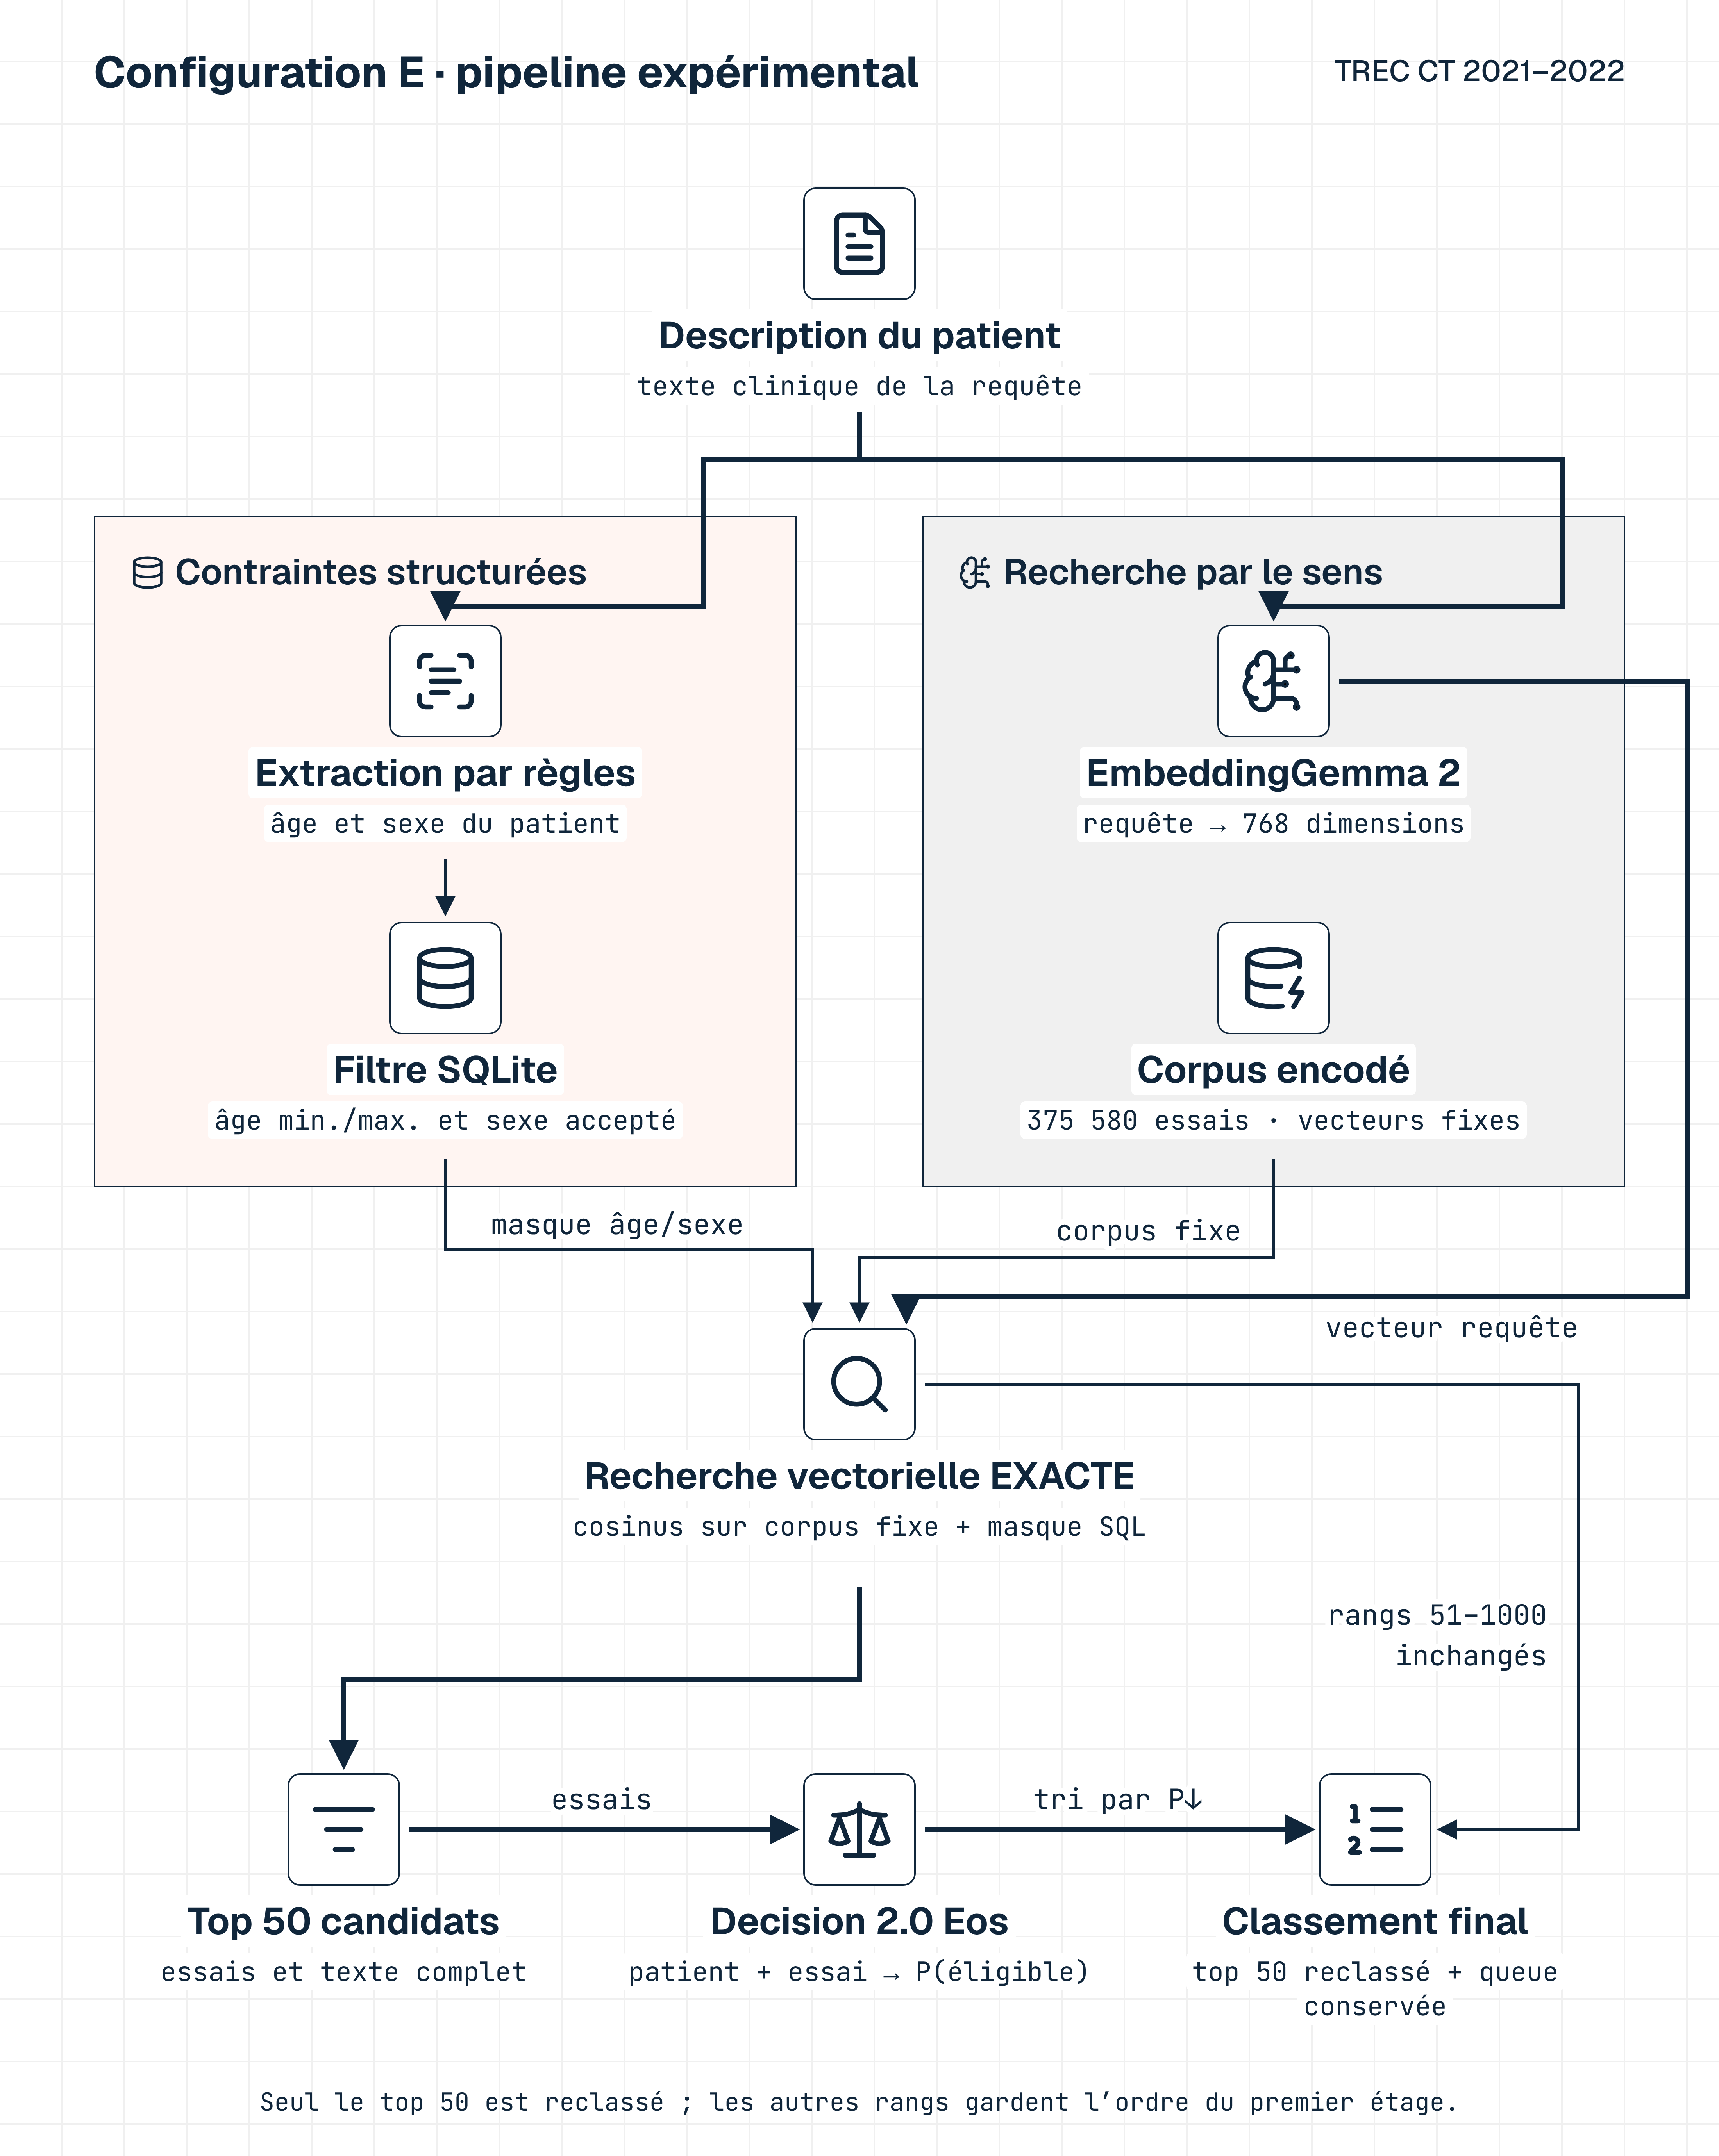
\includegraphics[width=\linewidth,height=45cm,keepaspectratio]{figures/pipeline-e-fr.png}
\caption{Configuration E : filtre âge/sexe, recherche exacte, puis reclassement Eos du top 50. Le modèle lit le patient et le texte de l'essai.}
\end{figure}
\end{block}
\begin{block}{Données et protocole}
TREC Clinical Trials : \textbf{375\,580 essais}, \textbf{75 requêtes en 2021} et \textbf{50 en 2022}. Les jugements distinguent les essais éligibles, exclus et non pertinents.

Le même corpus complet sert à toutes les configurations. Les résultats sont évalués jusqu'au rang 1\,000. La nDCG@10 utilise les trois niveaux ; les mesures de précision et de rappel ne considèrent comme pertinents que les essais éligibles.

Les moyennes sont accompagnées d'intervalles de confiance par bootstrap sur les requêtes. Les métriques ont été recoupées avec \texttt{ir\_measures}.
\end{block}
\begin{block}{Ablations : ce que chaque composant ajoute}
\begin{tabular}{@{}lp{0.76\linewidth}@{}}
\toprule
BM25 & Recherche lexicale sur le corpus complet. \\
A & Filtre SQL âge/sexe, puis BM25. \\
B & EmbeddingGemma 2, recherche vectorielle exacte. \\
C & Même recherche sémantique, avec filtre SQL âge/sexe. \\
D & Top-50 de B, reclassé par Eos. \\
E & Top-50 de C, reclassé par Eos. \\
\bottomrule
\end{tabular}

Le filtre conserve les essais sans contrainte renseignée. Le reclassement D/E garde les positions 51--1\,000 dans l'ordre du premier étage. Les jugements de pertinence ne sont jamais fournis aux modèles.
\end{block}
\begin{exampleblock}{Modèle de décision et témoin}
Decision 2.0 Eos (0,8B) répond par une probabilité d'éligibilité à une question oui/non portant sur un patient et un essai.

La même question oui/non est posée à chaque paire patient--essai, avec les critères d'éligibilité dans le texte. Les 50 candidats sont triés par probabilité décroissante ; les rangs suivants restent inchangés.

D/E sont mesurés : face à leur premier étage B/C, P@20 et R@20 progressent avec $p_{\mathrm{Holm}}<0{,}05$ les deux années. L'apport en nDCG@10 n'est pas concluant après correction ; le témoin BGE est désormais évalué.

{\small BGE-reranker-v2-m3 remplace Eos sur les mêmes pools (D$'$/E$'$). Ses logits ne sont pas des probabilités. 7\,340 paires calculées sur T4 en 8,34 minutes contre 91,80 pour Eos, sauvegardes comprises et hors chargement/préflight ; runtimes et précisions diffèrent. Aucune calibration clinique d'Eos n'est démontrée.}
\end{exampleblock}
\end{column}
\separatorcolumn
\begin{column}{\colwidth}
\begin{alertblock}{Résultats : l'apport d'Eos varie}
En 2021, la nDCG@10 passe de \textbf{0,396 à 0,402} pour B$\rightarrow$D et de \textbf{0,413 à 0,415} pour C$\rightarrow$E. En 2022 : \textbf{0,411 à 0,474} et \textbf{0,423 à 0,479}.

Ces hausses de moyennes ne sont pas concluantes en nDCG@10 après Holm dans la famille de 99 tests par année. Les améliorations de P@20 et R@20 face au premier étage sont concluantes les deux années ; Eos ne dépasse pas BGE de manière concluante en nDCG@10 après Holm.
\end{alertblock}
\begin{block}{Qualité de recherche : nDCG@10}
\begin{center}
\begin{tikzpicture}
\begin{axis}[width=0.96\linewidth,height=17cm,ybar,area legend,bar width=0.8cm,
 ymin=0,ymax=0.6,ytick={0,0.1,0.2,0.3,0.4,0.5,0.6},
 ylabel={nDCG@10},symbolic x coords={BM25,A,B,C,D,E},xtick=data,
 enlarge x limits=0.18,axis lines*=left,ymajorgrids=true,
 grid style={gray!20},legend style={at={(0.5,1.1)},anchor=south,legend columns=2,column sep=0.5cm,draw=none},legend cell align=left,
 tick label style={font=\small},label style={font=\small}]
\addplot[fill=nottblue,draw=nottblue] coordinates {(BM25,0.274678691228) (A,0.303322666333) (B,0.395518817183) (C,0.413314160455) (D,0.401778090295) (E,0.415292376176)};
\addplot[fill=gray!45,draw=gray!70] coordinates {(BM25,0.253752980688) (A,0.277478652849) (B,0.411090513769) (C,0.422785505187) (D,0.473789448233) (E,0.479065069771)};
\legend{2021 (75 requêtes),2022 (50 requêtes)}
\end{axis}
\end{tikzpicture}
\end{center}
{\small Moyennes ; intervalles de confiance à 95\,\% ci-dessous.}

{\small\begin{tabular*}{\linewidth}{@{\extracolsep{\fill}}lll@{}}
\toprule
Configuration & 2021 & 2022 \\
\midrule
BM25 & 0,275 [0,224 ; 0,327] & 0,254 [0,196 ; 0,316] \\
A : SQL + BM25 & 0,303 [0,251 ; 0,357] & 0,277 [0,214 ; 0,346] \\
B : sémantique & 0,396 [0,346 ; 0,445] & 0,411 [0,334 ; 0,492] \\
C : SQL + sémantique & 0,413 [0,361 ; 0,465] & 0,423 [0,346 ; 0,504] \\
D : B + Eos & 0,402 [0,350 ; 0,454] & 0,474 [0,405 ; 0,541] \\
E : C + Eos & 0,415 [0,363 ; 0,469] & 0,479 [0,413 ; 0,544] \\
D$'$ : B + BGE & 0,376 [0,325 ; 0,425] & 0,413 [0,337 ; 0,491] \\
E$'$ : C + BGE & 0,393 [0,339 ; 0,446] & 0,420 [0,345 ; 0,497] \\
\bottomrule
\end{tabular*}}


{\small\begin{tabular*}{\linewidth}{@{\extracolsep{\fill}}llll@{}}
\toprule
Année & Paire & $\Delta$ nDCG@10 [IC 95\,\%] & $p_{\mathrm{Holm}}$ \\
\midrule
2021 & D--B & $0{,}0063\;[-0{,}0365, 0{,}0492]$ & 1,000 \\
2021 & E--C & $0{,}0020\;[-0{,}0425, 0{,}0462]$ & 1,000 \\
2021 & E--D & $0{,}0135\;[-0{,}0045, 0{,}0339]$ & 1,000 \\
2022 & D--B & $0{,}0627\;[0{,}0055, 0{,}1146]$ & 0,416 \\
2022 & E--C & $0{,}0563\;[-0{,}0004, 0{,}1076]$ & 0,747 \\
2022 & E--D & $0{,}0053\;[-0{,}0121, 0{,}0243]$ & 1,000 \\
\bottomrule
\end{tabular*}}

{\small Wilcoxon pairé ; 99 tests observés par année, aucun emplacement réservé. E--E$'$ : R@20 progresse les deux années ; P@20 et R@10 progressent aussi en 2022. Judged@10 hors famille. 10\,000 valeurs de métriques recoupées avec \texttt{ir\_measures}.}
\end{block}
\begin{exampleblock}{Robustesse : fautes dans les requêtes}
À 5\,\% puis 10\,\% de mots bruités, l'âge est correct pour \textbf{114/125} puis \textbf{102/125} requêtes ; le sexe pour \textbf{124/125} puis \textbf{123/125}. Un seul tirage synthétique imbriqué, graine 20261117 ; règles inchangées, chiffres, ponctuation et corpus intacts.

{\small\begin{tabular*}{\linewidth}{@{\extracolsep{\fill}}llrlll@{}}
\toprule
Année & Syst. & Bruit & Propre & Bruité & $\Delta$ [IC 95\,\%] \\
\midrule
    2021 & B & 5\% & 0{,}3955 & 0{,}3913 & $-0{,}0043\;[-0{,}0237, 0{,}0147]$ \\
    2021 & B & 10\% & 0{,}3955 & 0{,}3816 & $-0{,}0139\;[-0{,}0355, 0{,}0065]$ \\
    2021 & C & 5\% & 0{,}4133 & 0{,}4077 & $-0{,}0056\;[-0{,}0245, 0{,}0126]$ \\
    2021 & C & 10\% & 0{,}4133 & 0{,}4003 & $-0{,}0130\;[-0{,}0354, 0{,}0089]$ \\
    \midrule
    2022 & B & 5\% & 0{,}4111 & 0{,}3925 & $-0{,}0185\;[-0{,}0347, -0{,}0036]$ \\
    2022 & B & 10\% & 0{,}4111 & 0{,}3839 & $-0{,}0272\;[-0{,}0499, -0{,}0067]$ \\
    2022 & C & 5\% & 0{,}4228 & 0{,}4130 & $-0{,}0097\;[-0{,}0281, 0{,}0084]$ \\
    2022 & C & 10\% & 0{,}4228 & 0{,}3952 & $-0{,}0276\;[-0{,}0525, -0{,}0049]$ \\
\bottomrule
\end{tabular*}}

{\small nDCG@10 moyenne et différence absolue bruité--propre avec IC bootstrap pairé à 95\,\%. B/C : 5\,000 valeurs recoupées avec \texttt{ir\_measures}.}

En 2022, B perd ponctuellement 4,51\,\% puis 6,62\,\% ; C, 2,30\,\% puis 6,53\,\%. Trois IC sont entièrement négatifs : B en 2022 aux deux niveaux et C à 10\,\%. Les cinq autres IC B/C incluent zéro, comme les huit IC BM25/A. Aucune comparaison directe de sensibilité B--C ni test corrigé n'est effectué.

Ces mesures ne démontrent pas une robustesse générale. Eos et BGE sur leurs propres pools bruités restent à mesurer.
\end{exampleblock}
\begin{block}{Limites de l'interprétation}
Les jugements TREC sont incomplets. Le top-10 sémantique contient davantage de documents non jugés que BM25 ; les scores ne décrivent donc pas parfaitement toute la pertinence retrouvée.

Un filtre strict peut éliminer un essai éligible. L'extraction âge/sexe a été développée sur ces mêmes 125 requêtes : sa réussite sur les requêtes propres ne mesure pas une généralisation à de nouveaux patients.

Les données sont en anglais. Aucune validation en français, en milieu hospitalier congolais ou sur des données privées n'est présentée. Colab est un environnement cloud.
\end{block}
\begin{block}{Perspectives}
Mesurer la sensibilité d'Eos et de BGE aux fautes de frappe, puis valider le français et l'exécution locale. Les résultats actuels ne démontrent pas une supériorité générale d'Eos sur BGE. Étendre ensuite le protocole à la recherche texte--image avec IU Chest X-ray ; cette expérience radiologique est une perspective, sans résultat dans cette étude.
\end{block}
\begin{block}{Code, résultats et reproductibilité}
\begin{minipage}[c]{0.80\linewidth}
{\small TREC Clinical Trials 2021--2022 (NIST). Code, scores Eos/BGE, versions des modèles, empreintes et protocole : dépôt public du projet.\par\smallskip
\href{https://github.com/Tresorkaseka/hybrid-medical-ir-indaba}{\texttt{github.com/Tresorkaseka/}}\par
\href{https://github.com/Tresorkaseka/hybrid-medical-ir-indaba}{\texttt{hybrid-medical-ir-indaba}}}
\end{minipage}\hfill
\begin{minipage}[c]{0.17\linewidth}
\centering
\qrcode[height=3.7cm]{https://github.com/Tresorkaseka/hybrid-medical-ir-indaba}
\end{minipage}
\end{block}
\end{column}
\separatorcolumn
\end{columns}
\end{frame}
\end{document}
